\documentclass[border=10pt]{standalone}

\usepackage{tikz}
\usepackage{tikzsymbols}
\usetikzlibrary{calc,patterns,shapes.geometric}

\def\centerarc[#1](#2)(#3:#4:#5){\draw[#1] ($(#2)+({#5*cos(#3)},{#5*sin(#3)})$) arc (#3:#4:#5);}

\begin{document}
	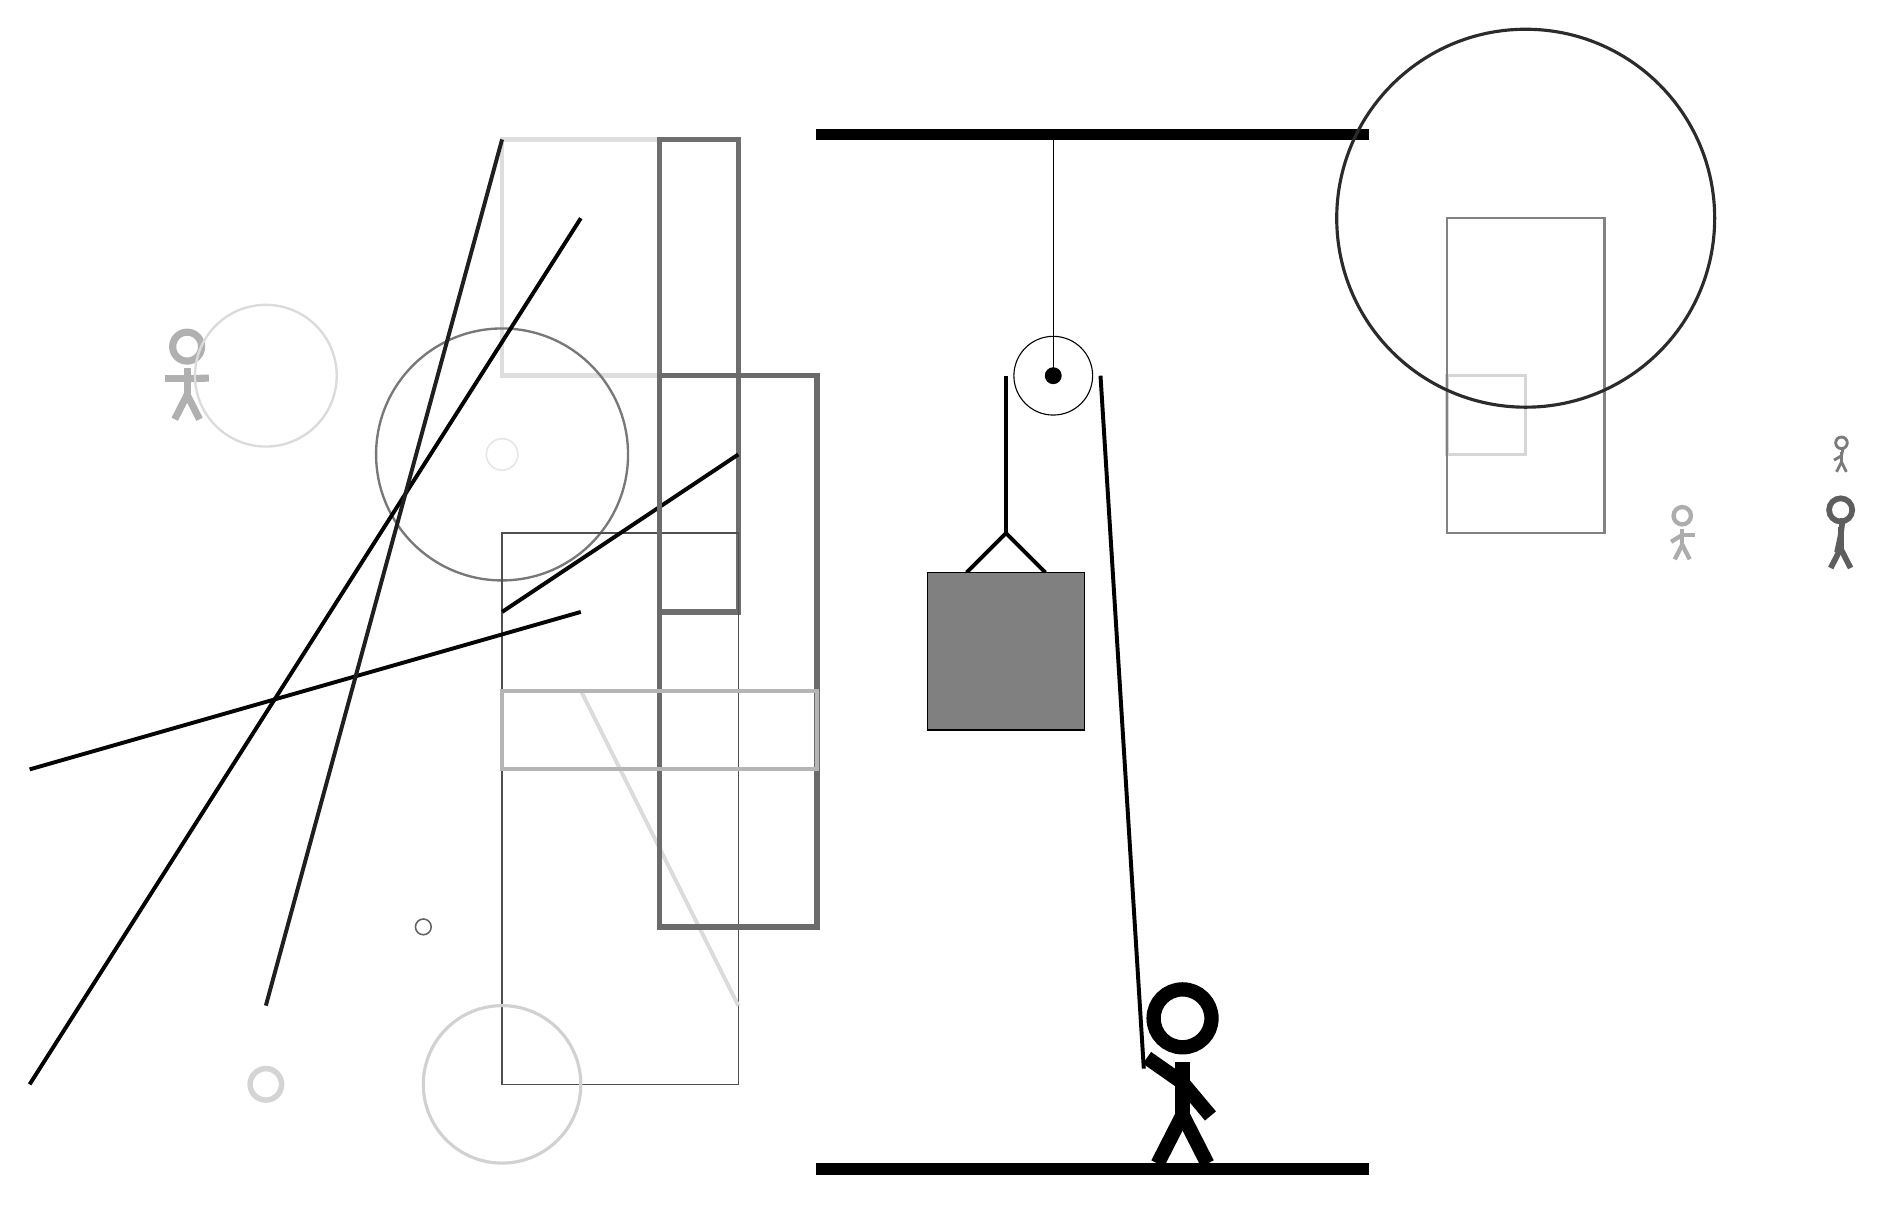
\begin{tikzpicture}
		%%%%% START %%%%%
		
		\draw[fill=black] (-2, 10) rectangle (5, 10.125);
		
		\draw (1, 7) circle (0.5);
		\draw[fill=black] (1, 7) circle (0.1);
		\draw (1, 10) -- (1, 7);
		
		\node[line width=0.6mm, color=black!31] at (-10, 7) {\Strichmaxerl[5][0][2]};
		
		\draw[line width=0.6mm, color=black!13] (-4, 7) rectangle (-6, 10);
		\node[line width=0.6mm, color=black!63] at (11, 5) {\Strichmaxerl[4][78][83]};
		\draw[line width=0.4mm, color=black!16] (7, 6) rectangle (6, 7);
		
		\draw [line width=0.3mm, color=black!53](-6, 6) circle (1.6);
		
		\draw [line width=0.2mm, color=black!10](-6, 6) circle (0.2);
		\draw[line width=0.3mm, color=black!49] (6, 9) rectangle (8, 5);
		
		\draw [line width=0.4mm, color=black!83](7, 9) circle (2.4);
		\draw [line width=0.3mm, color=black!14](-9, 7) circle (0.9);
		
		\draw[line width=0.7mm, color=black!57] (-3, 4) rectangle (-4, 10);
		\draw[line width=0.2mm, color=black!69] (-3, 5) rectangle (-6, -2);
		\draw[line width=0.5mm, color=black!97](-3, 6) -- (-6, 4);
		\draw[line width=0.5mm, color=black!98](-5, 4) -- (-12, 2);
		\draw[line width=0.5mm, color=black!14](-3, -1) -- (-5, 3);
		\draw [line width=0.7mm, color=black!17](-9, -2) circle (0.2);
		\draw [line width=0.2mm, color=black!61](-7, 0) circle (0.1);
		
		\draw[line width=0.5mm, color=black!99](-5, 9) -- (-12, -2);
		\draw[line width=0.7mm, color=black!58] (-2, 0) rectangle (-4, 7);
		\draw[line width=0.5mm, color=black!29] (-2, 3) rectangle (-6, 2);
		\node[line width=0.6mm, color=black!32] at (9, 5) {\Strichmaxerl[3][31][0]};
		\draw[line width=0.3mm, color=black!80] (-3, 1) rectangle (-3, 1);
		\draw [line width=0.4mm, color=black!18](-6, -2) circle (1.0);
		\node[line width=0.3mm, color=black!52] at (11, 6) {\Strichmaxerl[2][31][78]};
		\draw[line width=0.5mm, color=black!88](-6, 10) -- (-9, -1);
		
		\draw[line width=0.5mm] (-0.1, 4.5) -- (0.4, 5.0) -- (0.9, 4.5);
		\draw[fill=black!50] (-0.6, 4.5) rectangle (1.4, 2.5);
		
		\draw[line width=0.5mm] (0.4, 7) -- (0.4, 5.0);
		\centerarc[line width=0.5mm](1, 7)(0:180:0.6);
		\draw[line width=0.5mm](1.6, 7) -- (2.15, -1.8);
		
		\node at (2.6, -1.9) {\Strichmaxerl[10][-35][-50]};
		
		\draw[fill=black] (-2, -3) rectangle (5, -3.15);
		
		%%%%% END %%%%%
	\end{tikzpicture}
\end{document}